\section{Literature Retrieval and Abstract Screening}
\label{sec:retrieval_screening}

\subsection{Multi-Provider Retrieval and Metadata Cleaning}
Literature discovery (\texttt{providers.py}) queries multiple bibliographic APIs using structured boolean queries pairing oligopeptide length terms (\texttt{tetrapeptide} through \texttt{eicosapeptide}/\texttt{icosapeptide}) with self-assembly morphology keywords (\texttt{nanostructure}, \texttt{nanotube}, \texttt{nanofiber}, \texttt{nanorod}, \texttt{hydrogel}, \texttt{nanosphere}, \texttt{nanoparticle}, \texttt{self-assembly}), filtered to English primary research articles where supported:
\begin{itemize}
    \item \textbf{NCBIProvider}: Queries PubMed and PubMed Central (PMC) via E-Utilities (\texttt{esearch}/\texttt{efetch}) with API key authentication, batching (100--150 IDs per request), and rate-limit delays.
    \item \textbf{ScopusProvider}: Queries the Elsevier Scopus Search API for title/abstract/keyword metadata.
    \item \textbf{OpenAlexProvider} and \textbf{SemanticScholarProvider}: Provide auxiliary metadata, DOI-based abstract backfilling (\texttt{find\_abstracts\_by\_doi}), and Open Access PDF URL discovery.
\end{itemize}
Following ingestion, \texttt{deduplicate\_by\_doi()} normalizes DOIs and removes duplicate records, \texttt{find\_abstracts\_by\_doi()} backfills missing abstracts via OpenAlex, and \texttt{remove\_empty\_abstract\_title\_papers()} prunes entries lacking usable metadata. For papers marked \texttt{PaperStatus.USABLE}, \texttt{fetch\_paper\_fulltexts()} retrieves PMC JATS~XML first and falls back to OpenAlex PDFs, storing payloads in Azure Blob Storage (\texttt{azure\_storage.py}) with local caching.

\subsection{Stage 1: High-Recall Abstract Relevance Screening}
Before downloading full texts, \texttt{relevance.py} triages \texttt{not\_processed} papers using only their title and abstract. Screening supports both single-paper mode (\texttt{screen\_papers}) and batched bulk mode (\texttt{bulk\_screen\_papers}, default \texttt{batch\_size=50}), returning structured \texttt{RelevanceResult} objects containing \texttt{detected\_clues}, \texttt{explanation}, \texttt{is\_relevant}, and \texttt{confidence} $\in [0.0, 1.0]$.

The system prompt explicitly prioritizes \textbf{high recall}: borderline wet-lab papers are retained as relevant (with lower confidence), and only unambiguously out-of-scope studies---purely computational/theoretical papers without experimental validation, review articles, or studies exclusively on intact full-length proteins---are discarded.

\begin{table}[htbp]
\centering
\caption{Abstract screening recall on 1,000 sampled papers across LLM backends.}
\label{tab:relevance_recall}
\begin{tabular}{@{}lcc@{}}
\toprule
\textbf{Model} & \textbf{Recall} & \textbf{Run Identifier} \\
\midrule
Llama 3.2 3B & 0.970 & \texttt{1794483970} \\
Gemini 3.5 Flash Lite & 0.886 & \texttt{1794437084} \\
Gemini 3.1 Flash Lite & 0.873 & \texttt{1794437892} \\
DeepSeek R1 8B & 0.816 & \texttt{1794491078} \\
\bottomrule
\end{tabular}
\end{table}

On a 119-paper golden benchmark subset, Gemini~3.5~Flash~Lite and Gemma~31B each retained 118/119 papers, while Llama~3.2~3B retained 115/119. Across a 1,000-paper recall sample (\Cref{tab:relevance_recall}), Llama~3.2~3B achieved the highest recall ($0.970$) at zero API cost via local Ollama inference, making it suitable for large-scale pre-filtering. Applied to the full $\sim$50,020-paper scraped corpus, Llama~3.2~3B classified 28,664 papers as relevant and filtered out 21,356 non-relevant papers ($42.7\%$ reduction in downstream full-text processing). \Cref{fig:relevance_conf} compares confidence score distributions between Gemini and Llama~3.2~3B on large screening runs.

\begin{figure}[htbp]
\centering
\begin{subfigure}[b]{0.48\textwidth}
    \centering
    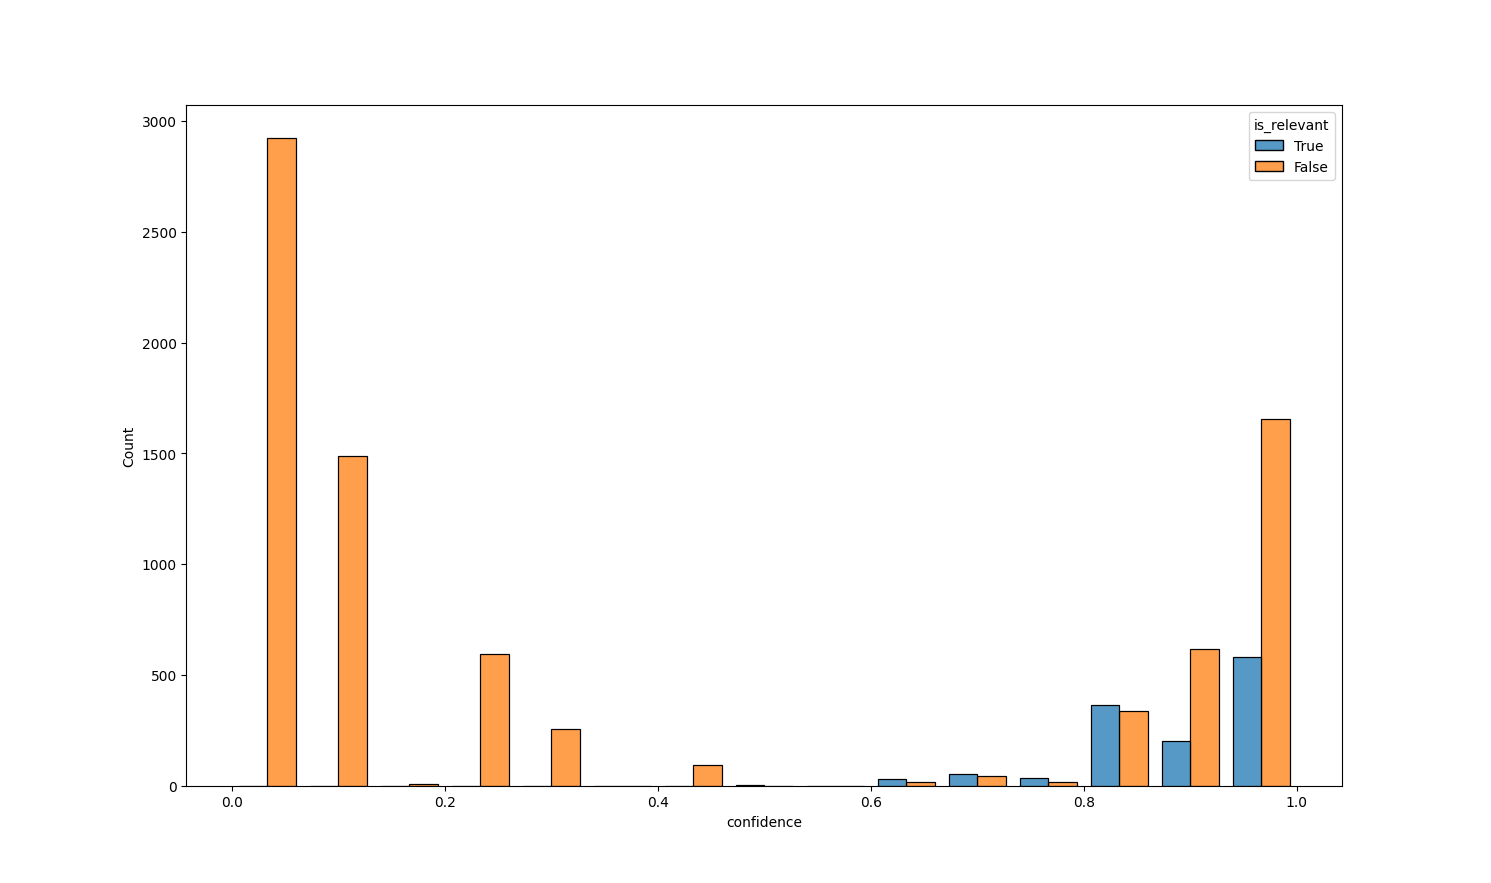
\includegraphics[width=\textwidth]{confidence-gemini-10k.png}
    \caption{Gemini (10k-paper run)}
    \label{fig:conf_gemini}
\end{subfigure}
\hfill
\begin{subfigure}[b]{0.48\textwidth}
    \centering
    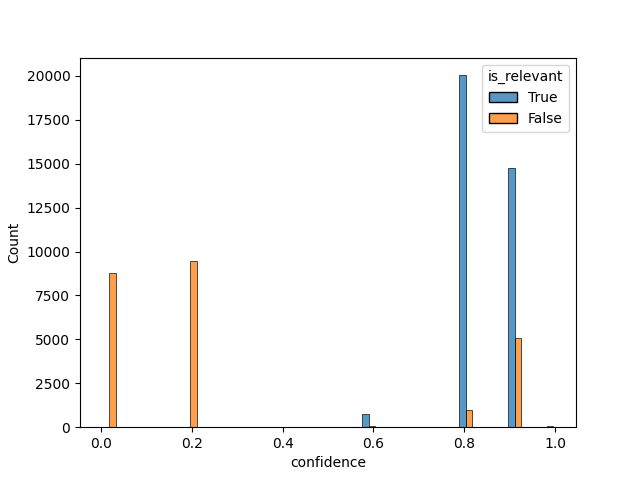
\includegraphics[width=\textwidth]{confidence-llama-complete.png}
    \caption{Llama 3.2 3B (full corpus)}
    \label{fig:conf_llama}
\end{subfigure}
\caption{Abstract relevance screening confidence distributions across models.}
\label{fig:relevance_conf}
\end{figure}
